\documentclass[tikz,border=10pt]{standalone}
\usepackage{tikz}
\usetikzlibrary{shapes.geometric, arrows.meta, positioning, calc, fit, backgrounds}

\begin{document}
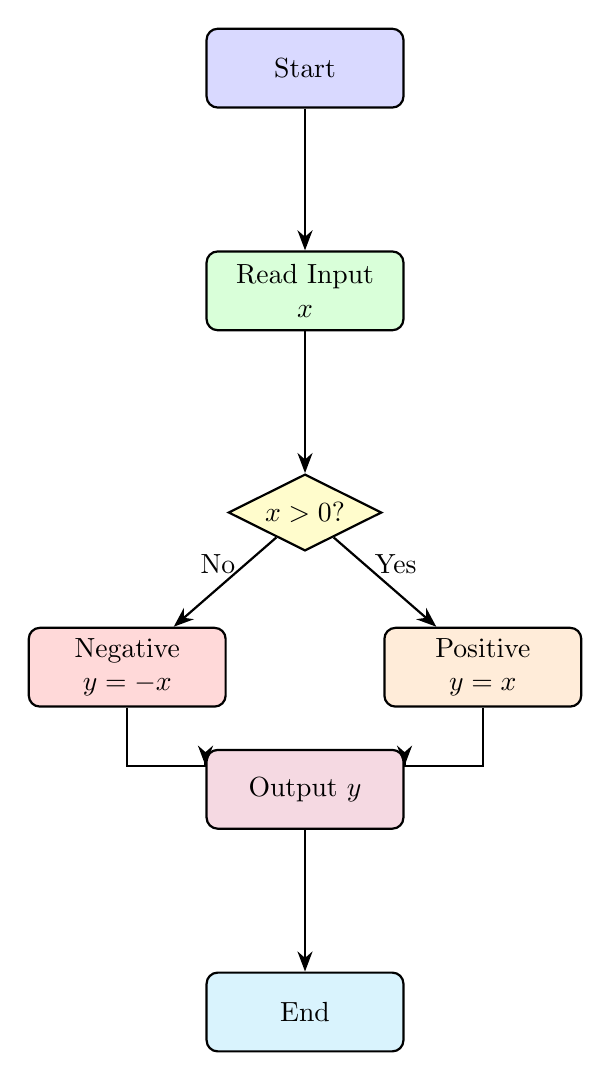
\begin{tikzpicture}[
    node distance=1.8cm and 2.5cm,
    process/.style={rectangle, draw, thick, minimum width=2.5cm, minimum height=1cm, align=center, rounded corners=4pt, fill=white},
    decision/.style={diamond, draw, thick, aspect=2, align=center, fill=yellow!20, inner sep=2pt},
    arrow/.style={-{Stealth[scale=1.1]}, thick, >=stealth}
]

% Nodes
\node[process, fill=blue!15] (start) {Start};
\node[process, fill=green!15, below=of start] (input) {Read Input\\$x$};
\node[decision, below=of input] (check) {$x > 0$?};
\node[process, fill=red!15, below left=1.2cm and 0.5cm of check] (neg) {Negative\\$y = -x$};
\node[process, fill=orange!15, below right=1.2cm and 0.5cm of check] (pos) {Positive\\$y = x$};
\node[process, fill=purple!15, below=2.5cm of check] (output) {Output $y$};
\node[process, fill=cyan!15, below=of output] (end) {End};

% Arrows
\draw[arrow] (start) -- (input);
\draw[arrow] (input) -- (check);
\draw[arrow] (check) -- node[left, pos=0.3] {No} (neg);
\draw[arrow] (check) -- node[right, pos=0.3] {Yes} (pos);
\draw[arrow] (neg) |- ([yshift=0.3cm]output.west) -- (output);
\draw[arrow] (pos) |- ([yshift=0.3cm]output.east) -- (output);
\draw[arrow] (output) -- (end);

\end{tikzpicture}
\end{document}
